\documentclass[11pt]{article}
\usepackage[utf8]{inputenc}
\usepackage[T1]{fontenc}
\usepackage{lmodern}
\IfFileExists{spanish.ldf}{\usepackage[spanish,es-noshorthands,es-tabla]{babel}}{%
  \renewcommand{\abstractname}{Resumen}\renewcommand{\tablename}{Tabla}%
  \renewcommand{\figurename}{Figura}\renewcommand{\refname}{Referencias}}
\emergencystretch=3em
\usepackage[margin=1in]{geometry}
\usepackage{amsmath,amssymb,booktabs,graphicx,hyperref,enumitem}
\hypersetup{colorlinks=true,linkcolor=blue,citecolor=blue,urlcolor=blue}

\title{Escribir capacidades nuevas a mano en un modelo de lenguaje preentrenado}
\author{Nombre del autor\\ Afiliación\\ \texttt{correo}}
\date{Noviembre de 2026}

\begin{document}
\maketitle

\begin{abstract}
Mostramos que un modelo de lenguaje grande (LLM), razonando sobre lo que debe calcular cada parte de una red, puede escribir a mano pesos que dan a un modelo de lenguaje preentrenado pequeño capacidades que no tenía, sin descenso de gradiente y sin datos de entrenamiento. El modelo receptor es stories15M, un modelo de 15M de parámetros con arquitectura Llama 2, entrenado solo con cuentos infantiles, que obtiene un 0\,\% en aritmética de varios dígitos y no conoce ninguno de los hechos que le enseñamos. Primero, un circuito de 7 capas escrito a mano, injertado junto al modelo congelado, lee los tokens tal cual y lleva el benchmark de aritmética de GPT-3 del 0\,\% al 100\,\% en los ocho subconjuntos de suma y resta (16\,000 problemas; 20\,000 de 20\,000 en una comprobación exhaustiva), sin cambiar, de forma demostrable, ninguna otra salida. Segundo, editando solo pesos que el modelo ya tiene, le enseñamos siete capitales de países que nunca ha visto (del 0\,\% al 91\,\% en paráfrasis nuevas) y la suma de dos dígitos (del 12\,\% al 52\,\% de respuestas exactas en plantillas nuevas). Por el camino descubrimos que los tokens raros son casi indistinguibles para el modelo (coseno entre embeddings de 0,96 a 0,999), lo que hay que reparar antes de poder escribir ningún conocimiento, e introducimos un código angular para números que es invariante a la normalización RMS. Los resultados respaldan una afirmación sencilla: los pesos escritos a mano pueden añadir capacidades a un modelo preentrenado, no solo eliminar obstáculos a las que ya tiene.
\end{abstract}

\section{Introducción}
Los pesos de una red neuronal los escribe casi siempre un optimizador. Un modelo adquiere una capacidad viendo datos y siguiendo un gradiente, y las ediciones de modelos entrenados suelen quitar o redirigir lo que ya existe. Un trabajo reciente sobre \emph{programación en el espacio de pesos} \cite{takehi2026} mostró que un LLM de frontera puede leer y editar los pesos de otras redes, y dejó abierta la pregunta de si esas ediciones pueden añadir una capacidad que el modelo no tiene.

Estudiamos esa pregunta en un modelo lo bastante pequeño como para inspeccionarlo por completo. stories15M nunca ha visto aritmética ni geografía: a ``The capital of France is'' responde ``a very special person'' y a ``2 + 3 ='' responde con un cuento. Nos preguntamos si un LLM, escribiendo pesos directamente a partir de su comprensión del modelo y del algoritmo deseado, puede darle esas capacidades. Puede, en dos escenarios:
\begin{itemize}[leftmargin=*]
\item \textbf{Injerto.} Un transformer pequeño, escrito por completo a mano, funciona junto al modelo congelado y suma sus logits. Tiene que encontrar la pregunta en los tokens, leer los operandos como números, calcular el resultado y dar formato a la respuesta. Resuelve de forma exacta el benchmark de aritmética de GPT-3 y no cambia nada más.
\item \textbf{Cirugía dentro de los pesos.} Solo cambian pesos existentes: se reescriben unas pocas filas del embedding, neuronas y filas de atención. El modelo aprende siete hechos nuevos y la suma de dígitos, con un coste medible pero moderado para su tarea original.
\end{itemize}

\paragraph{Contribuciones.}
\begin{enumerate}[leftmargin=*]
\item Un circuito escrito a mano que lleva un LM preentrenado del 0\,\% al 100\,\% en el benchmark de aritmética de GPT-3 (suma y resta, de 2 a 5 dígitos), exacto hasta operandos de 12 dígitos, con salidas demostrablemente intactas en cualquier otro texto (sección~\ref{sec:graft}).
\item Cirugía dentro de los pesos que escribe hechos nuevos (del 0\,\% al 91\,\% en paráfrasis nuevas) y aritmética nueva (del 12\,\% al 52\,\% de respuestas exactas) en los propios pesos del modelo (secciones~\ref{sec:facts}--\ref{sec:arith}).
\item Un diagnóstico: los tokens raros colapsan sobre un embedding compartido y resultan invisibles para el modelo; y una reparación que apenas cuesta nada (sección~\ref{sec:facts}).
\item Una pequeña caja de herramientas para escribir pesos bajo normalización RMS: números codificados como ángulos, etiquetas que viven una sola capa, canales de atención dedicados en pares RoPE liberados y sumideros de atención que hacen que las cabezas nuevas callen por defecto (sección~\ref{sec:toolkit}).
\end{enumerate}

\section{Marco experimental}
\paragraph{Modelo receptor.} stories15M \cite{llama2c}: arquitectura Llama 2 con 6 capas, 6 cabezas de tamaño 48, $d_\text{model}=288$, MLP SwiGLU de anchura 768, RMSNorm, RoPE, embeddings de entrada y salida ligados, y un vocabulario SentencePiece de 32\,000 tokens que separa los números en dígitos sueltos. Se entrenó solo con TinyStories \cite{tinystories}. Lo elegimos porque carece por completo de las capacidades objetivo, de modo que ninguna mejora puede deberse a desbloquear algo latente.

\paragraph{Reglas.} Ningún peso procede de descenso de gradiente, de un optimizador, de una búsqueda sobre pesos ni de un ajuste a etiquetas. Cada peso modificado lo escribe el autor con una función explícita: qué dirección lee, qué calcula y dónde escribe. En la sección~\ref{sec:graft} se añaden pesos nuevos junto al modelo; en las secciones~\ref{sec:facts}--\ref{sec:arith} solo cambian pesos existentes y la arquitectura no se toca.

\paragraph{El autor.} Todos los pesos los escribió Claude (Anthropic), trabajando en un entorno Python con 2 núcleos de CPU. El autor podía ejecutar pasadas hacia delante, y las usó de dos maneras: para medir las magnitudes que fijan direcciones y umbrales (medias de clase, covarianzas y proyecciones sobre un pequeño conjunto de plantillas de \emph{diseño}) y para comprobar. Direcciones como ``la lectura del país $k$'' son estadísticos en forma cerrada de pasadas hacia delante, no sondas entrenadas. Todos los umbrales, los dos pesos de mezcla de cada neurona ``Y'' de la sección~\ref{sec:facts} (elegidos de una pequeña rejilla) y las tres calibraciones de ganancia de la sección~\ref{sec:arith} se fijaron solo con plantillas de diseño.

\paragraph{Evaluación.} Evaluamos con plantillas nuevas, nunca usadas al escribir los pesos, y damos el acierto exacto con decodificación voraz. Cuando el espacio de entradas es pequeño comprobamos todos los casos. Para medir el daño damos la pérdida sobre texto de validación de TinyStories (modelo base: 1,0997 nats por token) e inspeccionamos generaciones libres.

\section{Injerto de aritmética exacta}\label{sec:graft}
Un transformer escrito a mano, colocado junto al modelo congelado, lo lleva del 0\,\% al 100\,\% en todos los subconjuntos de suma y resta del benchmark de aritmética de GPT-3 \cite{gpt3}, y deja todas las demás salidas exactamente como estaban.

\paragraph{Circuito.} 7 capas, 78 dimensiones residuales, 800 pesos distintos de cero, sin normalización. Solo ve la identidad de los tokens y la posición absoluta $i$; no recibe ninguna característica de la tarea. Sus logits se suman a los del LM, lo que equivale a ensanchar el modelo con dimensiones, cabezas y neuronas nuevas en bloques diagonales (figura~\ref{fig:graft}).

\begin{figure}[t]
\centering
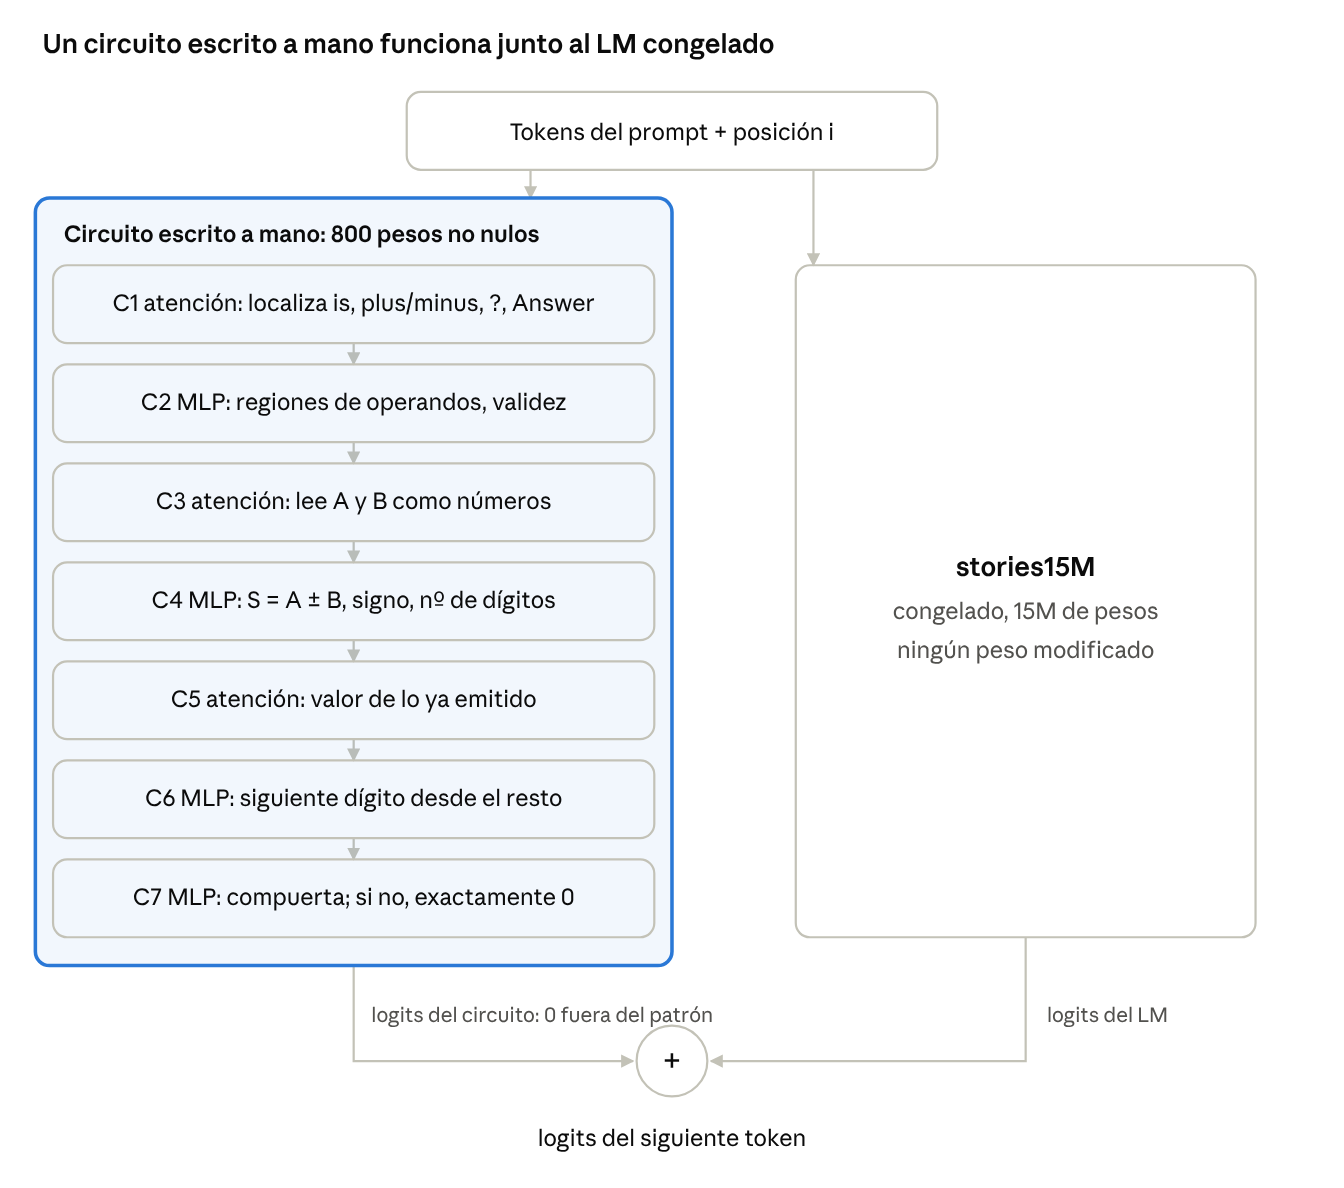
\includegraphics[width=0.82\linewidth]{fig_graft_es.png}
\caption{El modelo injertado: 7 capas escritas a mano junto a las 6 capas congeladas de stories15M.}
\label{fig:graft}
\end{figure}

\paragraph{Cómo calcula.} La atención de C1 localiza los últimos tokens \texttt{is}, \texttt{plus}/\texttt{minus}, \texttt{?} y \texttt{Answer}. C2 marca qué dígitos pertenecen a cada operando y comprueba la plantilla. C3 lee cada operando como un número exacto: pesos de atención proporcionales a 10 elevado a la significancia de cada dígito, normalizados frente a un sumidero fijo en el token BOS, devuelven el valor del operando multiplicado por una constante conocida. C4--C6 calculan $S=A\pm B$, su signo y su número de dígitos, restan el valor de los dígitos ya emitidos y eligen el siguiente dígito aplicando umbrales al resto. C7 escribe logits grandes para el espacio o el signo menos iniciales, cada dígito y un salto de línea final, y su salida es exactamente 0 siempre que la plantilla o la fase no encajan.

\begin{table}[h]
\centering
\small
\begin{tabular}{lccc}
\toprule
Subconjunto de aritmética de GPT-3 & Problemas & stories15M & + circuito \\
\midrule
Suma / resta de 2 dígitos & 2\,000 / 2\,000 & 0,0\,\% / 0,0\,\% & 100\,\% / 100\,\% \\
Suma / resta de 3 dígitos & 2\,000 / 2\,000 & 0,0\,\% / 0,0\,\% & 100\,\% / 100\,\% \\
Suma / resta de 4 dígitos & 2\,000 / 2\,000 & 0,0\,\% / 0,0\,\% & 100\,\% / 100\,\% \\
Suma / resta de 5 dígitos & 2\,000 / 2\,000 & 0,0\,\% / 0,0\,\% & 100\,\% / 100\,\% \\
Filas oficiales 0--99, suma / resta de 5 dígitos & 100 / 100 & 0,0\,\% / 0,0\,\% & 100\,\% / 100\,\% \\
Exhaustivo: todos los $a,b\in[0,99]$, suma y resta & 20\,000 & -- & 100\,\% \\
\bottomrule
\end{tabular}
\caption{Acierto exacto, decodificación voraz, sin ejemplos. Cada subconjunto de 2\,000 problemas da una cota inferior de Clopper--Pearson al 95\,\% de 99,82\,\%. Los 16\,000 problemas se regeneraron siguiendo el esquema de muestreo de GPT-3 (operandos uniformes por debajo de $10^N$, semillas fijas); las filas oficiales se obtuvieron de EleutherAI/arithmetic.}
\end{table}

\paragraph{Sin efectos secundarios.} En texto de validación de TinyStories, los logits del circuito son exactamente cero en todas las posiciones y la pérdida es idéntica (perplejidad 3,003201 con y sin injerto). Las generaciones voraces a partir de casi-aciertos como ``What is 3 plus 2? He did not know.'' coinciden token a token. Tras responder, el LM continúa con su propio texto: ante ``What is 7 minus 66?'' el modelo base escribe ``Mommy, what is that?'', mientras que el injertado escribe `` -59'' y un salto de línea, y luego sigue.

\paragraph{Más allá del benchmark.} El circuito sigue siendo exacto en problemas aleatorios de 6, 8, 10 y 12 dígitos (40 por configuración, suma y resta). Falla a los 13 dígitos por diseño, porque su tabla de potencias de diez llega hasta $10^{12}$.

\section{Cirugía dentro de los pesos I: hacer visibles los tokens raros y escribir hechos nuevos}\label{sec:facts}
Editando solo pesos que el modelo ya tiene, le enseñamos las capitales de siete países de los que nunca ha oído hablar. Responde correctamente hasta en un 91\,\% de las paráfrasis nuevas, desde un 0\,\%.

\paragraph{Diagnóstico: los tokens raros son invisibles.} Antes de escribir ningún hecho leemos los embeddings implicados. Seis de los siete tokens de país (Spain, Italy, Japan, Germany, England, Russia) y el token ``capital'' tienen similitudes coseno por pares entre 0,96 y 0,999; los siete tokens de capitales tienen al menos 0,93. Estos tokens nunca aparecieron en el entrenamiento, así que sus embeddings derivaron juntos. Para el modelo, ``Spain'' y ``Japan'' son la misma palabra, y ninguna edición posterior puede asociarles hechos distintos. Por eso el primer paso de la cirugía es hacerlos distinguibles.

\paragraph{Cirugía.}
\begin{enumerate}[leftmargin=*]
\item \textbf{Etiquetas.} Se añade un componente pequeño (norma 0,25) a 15 filas del embedding (7 países, ``capital'' y 7 capitales), cada uno en una dirección elegida para ser tranquila a la entrada y a la salida del modelo. Como los embeddings están ligados, una etiqueta grande cambiaría también los logits de salida; etiquetas y detectores juntos cambian la pérdida en cuentos en torno a un 0,2\,\%.
\item \textbf{Detectores.} 8 neuronas poco usadas del MLP de la capa 3 detectan la etiqueta de un país o de ``capital'' en el propio token y escriben allí una marca mayor.
\item \textbf{Canales de atención dedicados.} En las cabezas L4H3 y L4H4 vaciamos el par RoPE de baja frecuencia (44,\,45), lo que cuesta un 0,6\,\% de pérdida, y lo reutilizamos para que L4H3 atienda a las marcas de país y L4H4 a la de ``capital'', llevando ambas a la posición de la respuesta.
\item \textbf{Neuronas ``Y''.} 7 neuronas del MLP de la capa 4 se activan cuando coinciden la marca del país, la de la pregunta por la capital y una señal de hueco de respuesta, y escriben la capital mediante una dirección discriminante sobre el vocabulario.
\end{enumerate}

\begin{table}[h]
\centering
\small
\setlength{\tabcolsep}{4pt}\begin{tabular}{lccccc}
\toprule
Variante & Diseño & Paráfrasis & País no enseñado & Sin pregunta & Pérdida \\
\midrule
stories15M & 0\,\% & 0\,\% & 0\,\% & 0\,\% & 1,0997 \\
(a) ``Y'' por suma & 100\,\% & \textbf{91,4\,\%} & 65\,\% & 86\,\% & 1,1442 (+4,0\,\%) \\
(b) + canales ortogonales & 100\,\% & 80,0\,\% & \textbf{0\,\%} & 33\,\% & 1,1917 (+8,4\,\%) \\
(c) + hueco de respuesta & 100\,\% & 68,6\,\% & \textbf{0\,\%} & \textbf{4,8\,\%} & 1,1703 (+6,4\,\%) \\
\bottomrule
\end{tabular}
\caption{Hechos escritos en los propios pesos del modelo. ``País no enseñado'': produce una capital enseñada para uno de 5 países no enseñados. ``Sin pregunta'': produce una capital en frases que mencionan el país pero no preguntan por su capital. Diseño: 3 plantillas usadas para fijar direcciones; paráfrasis: 5 plantillas nunca vistas al escribir los pesos.}
\end{table}

Las variantes intercambian cobertura por precisión. La más estricta nunca inventa una capital para un país no enseñado y solo responde sin que se le pregunte en 1 de 21 frases, a costa de fallar paráfrasis cuyo hueco de respuesta difiere de las plantillas de diseño (``\ldots is called''). Las tres filas se reproducen con \texttt{facts7.py} con \texttt{variant} igual a a, b o c. Salidas típicas: ``The capital of France is'' $\to$ `` Paris''; ``In Italy, the capital city is'' $\to$ `` Rome''.

\section{Cirugía dentro de los pesos II: aritmética con código angular}\label{sec:arith}
De nuevo editando solo pesos existentes, enseñamos al modelo a sumar dos dígitos. En plantillas nuevas, sus respuestas exactas suben del 6\,\% al 28\,\% en total y del 12\,\% al 52\,\% en sumas hasta 9.

\paragraph{El obstáculo: la normalización.} RMSNorm reescala cada posición por un factor que depende del contexto, así que un número guardado como magnitud se distorsiona, y una cabeza de atención reparte su peso de forma desigual entre dos dígitos. Ambas cosas rompen la aritmética.

\paragraph{Código angular.} Guardamos el dígito $d$ como un vector de norma constante,
\begin{equation}
v_d = K\,(\cos d\phi,\ \sin d\phi,\ 1), \qquad \phi=\pi/24,
\end{equation}
como hace RoPE con las posiciones. La normalización no puede distorsionarlo, la tercera componente da a todos los dígitos la misma clave de atención, y la media de $v_a$ y $v_b$ apunta exactamente al ángulo $(a+b)\phi/2$. Leer la suma solo requiere entonces pruebas de semiplano $Y\cos\beta - X\sin\beta \ge 0$, que son homogéneas y, por tanto, insensibles a la escala.

\paragraph{Cirugía.}
\begin{enumerate}[leftmargin=*]
\item 20 neuronas de la capa 0 detectan cada dígito y escriben una etiqueta pequeña de tipo uno-de-N.
\item 20 neuronas de la capa 4 re-detectan la etiqueta y escriben el vector angular grande, de modo que la señal grande solo existe entre las capas 4 y 5.
\item La cabeza L5H5, la más barata de quitar de la última capa (+0,9\,\% de pérdida al anularla), se reconvierte por completo. Atiende solo a los dígitos, por igual, y a un sumidero en el token BOS cuando no hay ninguno; las salidas se eligen para que el sumidero no aporte casi nada.
\item En el MLP de la capa 5, 3 neuronas cancelan el vector grande en la propia posición del dígito (sus tres ganancias de salida son escalares calibrados con las apariciones de dígitos en el diseño), y 38 neuronas implementan 18 pruebas de semiplano sobre el ángulo más una prueba de presencia, que juntas eligen el dígito de la respuesta, condicionadas al hueco de respuesta.
\end{enumerate}

La cabeza reconvertida calcula el ángulo con precisión: en una variante de diagnóstico del circuito, la suma leída directamente de su salida en prompts de diseño fue 6,95 para 3+4, 18,00 para 9+9 y 2,22 para 2+0.

\begin{table}[h]
\centering
\begin{tabular}{lcc}
\toprule
40 pares de dígitos aleatorios & stories15M & Operado \\
\midrule
Respuesta exacta, plantillas de diseño & 7,5\,\% & \textbf{33,3\,\%} \\
Respuesta exacta, 4 plantillas nuevas & 6,3\,\% & \textbf{27,5\,\%} \\
Respuesta exacta, plantillas nuevas, sumas $\le 9$ & 11,9\,\% & \textbf{52,4\,\%} \\
Primer token, plantillas nuevas & 14,4\,\% & 73,1\,\% \\
Pérdida en cuentos & 1,0997 & 1,1603 (+5,5\,\%) \\
\bottomrule
\end{tabular}
\caption{Suma de dos dígitos escrita en los propios pesos del modelo.}
\end{table}

El acierto del primer token exagera el éxito, porque el primer token de cualquier suma de 10 a 18 es ``1''; la respuesta exacta es la medida honesta. Las pérdidas principales se producen después de la cabeza: el MLP final tiene que leer el ángulo desde una posición que también lleva otras señales, y en las sumas de dos cifras todavía no produce el segundo dígito.

\section{Una caja de herramientas para escribir pesos a mano}\label{sec:toolkit}
La mayoría de los intentos fallidos de este trabajo tuvieron las mismas pocas causas. Las técnicas de la tabla~\ref{tab:toolkit} son las que los resolvieron, y esperamos que se transfieran a otros modelos.

\begin{table}[h]
\centering
\small
\begin{tabular}{p{0.19\linewidth}p{0.32\linewidth}p{0.39\linewidth}}
\toprule
Técnica & Problema que resuelve & Cómo \\
\midrule
Leer antes de escribir & Las ediciones fallan en silencio si el modelo no puede representar las entradas & Comprobar que los tokens implicados tienen embeddings distinguibles; si no, repararlos con etiquetas pequeñas \\
Direcciones tranquilas & Las señales nuevas interfieren con lo que el modelo ya hace & Escribir en direcciones con momento de segundo orden bajo en la capa que las lee y poca energía en los logits de salida \\
Códigos de norma constante & RMSNorm reescala las magnitudes en cada posición & Codificar los valores como ángulos sobre un círculo más una componente constante de presencia \\
Pruebas homogéneas & Los umbrales se desplazan con la escala de la normalización & Comparar dos lecturas entre sí (pruebas de semiplano) en lugar de con una constante \\
Marcas de una sola capa & Las señales grandes corrompen todas las capas que atraviesan & Escribir pronto una etiqueta pequeña, amplificarla justo antes de la capa que la lee y cancelarla justo después \\
Canales de atención dedicados & La atención natural no mira donde el circuito lo necesita & Vaciar un par RoPE de baja frecuencia en una cabeza ($\approx$0,6\,\% de coste) y usarlo para una puntuación solo de contenido \\
Sumideros de atención & Una cabeza nueva escribe ruido cuando no están sus objetivos & Dar a BOS una puntuación fija menor y elegir direcciones de valor en las que BOS valga cero \\
Sustitutos del sesgo & Las capas de Llama no tienen sesgos & Usar una dirección cuya proyección es casi constante entre tokens ($\pm$6\,\%), calculada como $\Sigma^{-1}\mu$ \\
Escalones recortados & SiLU tiene fugas por debajo de cero y crece sin límite & Emparejar dos neuronas, $\mathrm{silu}(sx)-\mathrm{silu}(sx-10)$, para una salida en $[0,10]$ \\
\bottomrule
\end{tabular}
\caption{Técnicas que hicieron funcionar los pesos escritos a mano bajo normalización RMS.}
\label{tab:toolkit}
\end{table}

\section{Trabajo relacionado}
\paragraph{Programación en el espacio de pesos.} Takehi et al.\ \cite{takehi2026} acuñaron el término para un LLM de propósito general que lee y escribe directamente los pesos de una red. Identifican con qué se entrenaron redes pequeñas, reparan una política de control que fallaba, escriben desde cero políticas para juegos y editan el 0,016\,\% de los pesos de Qwen3.5-0.8B para eliminar un bucle de repetición, subiendo MATH-500 del 7,9\,\% al 48,1\,\%. No encontraron una mejora comparable en Gemma 3 270M y sugirieron que las ediciones de pesos eliminan obstáculos en vez de añadir capacidades. Nuestro trabajo es una continuación directa de esa pregunta abierta, con capacidades más estrechas y un modelo más pequeño.

\paragraph{Transformers compilados y escritos a mano.} Tracr \cite{tracr} compila programas RASP \cite{rasp} a pesos de transformer; AdderBoard \cite{adderboard} recopila transformers escritos a mano que suman números de 10 dígitos con apenas 5 parámetros. Construyen redes independientes; nosotros escribimos circuitos que viven dentro o al lado de un modelo preentrenado y tienen que convivir con él.

\paragraph{Edición de modelos.} ROME \cite{rome} y métodos afines cambian hechos concretos mediante actualizaciones en forma cerrada de pesos de MLP, normalmente sobre hechos que el modelo ya puede representar. Nuestros hechos tratan de tokens que el modelo no distingue al principio, y nuestra edición aritmética añade un algoritmo, no una asociación.

\paragraph{Aritmética en transformers.} El acoplamiento de posiciones \cite{cho2024} y los embeddings Abacus \cite{mcleish2024} ayudan a transformers entrenados a generalizar la aritmética a entradas más largas. Nuestro código angular está emparentado en espíritu con los embeddings de posición rotatorios, aplicados a valores en lugar de a posiciones.

\section{Limitaciones y próximos pasos}
\begin{itemize}[leftmargin=*]
\item \textbf{Capacidades estrechas, un solo modelo pequeño.} Siete hechos, suma de dígitos y aritmética con la plantilla del benchmark en un modelo de 15M de parámetros. Queda abierto si los métodos escalan a modelos mayores y habilidades más amplias.
\item \textbf{El injerto añade pesos.} La sección~\ref{sec:graft} ensancha el modelo con un bloque aparte; las secciones~\ref{sec:facts}--\ref{sec:arith} muestran la versión dentro de los pesos de la misma idea, con menor acierto.
\item \textbf{Dependencia de la plantilla.} El injerto lee una única plantilla de prompt; la edición de hechos dentro de los pesos falla con huecos de respuesta distintos de los de las plantillas de diseño.
\item \textbf{Efectos secundarios de la aritmética dentro de los pesos.} Tras escribir un número, el modelo editado a veces sigue con más dígitos, y en cuentos que contienen números puede colar un dígito donde no corresponde. La pérdida en cuentos (+5,5\,\%) no lo refleja, porque los cuentos de evaluación no contienen números. Una variante con una marca propia para el hueco de respuesta elimina esas fugas, pero todavía no hemos recuperado su precisión.
\item \textbf{Un autor, una sesión.} Todos los pesos los escribió un único LLM en una sola sesión de trabajo, con acceso a pasadas hacia delante. No hemos medido con qué fiabilidad otras sesiones u otros LLM llegan a los mismos resultados.
\item \textbf{Direcciones medidas.} Muchas direcciones son medias de clase y covarianzas de pasadas hacia delante sobre plantillas de diseño. Son estadísticos en forma cerrada, no parámetros entrenados, pero usan datos.
\end{itemize}
\paragraph{Próximos pasos.} Eliminar los efectos secundarios de la aritmética y producir sumas de dos cifras; escalar la edición de hechos a decenas de hechos y varias relaciones; repetir en un modelo mayor (stories42M, stories110M); y medir la fiabilidad entre sesiones independientes del autor.

\section*{Reproducibilidad}\sloppy
Todos los scripts se ejecutan en CPU en minutos, con semillas fijas. Injerto: \texttt{llama.py}, \texttt{circuit.py}, \texttt{eval.py}, \texttt{exhaustive\_graft.py}, \texttt{preserve.py}. Hechos: \texttt{surgery.py}, \texttt{facts6.py}, \texttt{facts7.py} (variantes a, b y c). Aritmética: \texttt{arith2.py}, \texttt{arith4.py}. Pesos de stories15M de la copia del checkpoint de Karpathy en \url{https://github.com/cgbur/llama2.zig}; filas del benchmark de \url{https://hf.co/datasets/EleutherAI/arithmetic}; cuentos de validación de \url{https://hf.co/datasets/roneneldan/TinyStories}.

\begin{thebibliography}{10}
\bibitem{takehi2026} R.~Takehi, J.~Teoh, A.~Zhang, O.~Khattab. Sparks of Weight-Space Programming: LLMs can natively read \& write neural network weights. Blog de MIT CSAIL, 2 de noviembre de 2026. \url{https://rikiyat.github.io/blog/weight-space-programming/}
\bibitem{gpt3} T.~Brown et al. Language Models are Few-Shot Learners. arXiv:2005.14165, 2020.
\bibitem{tinystories} R.~Eldan, Y.~Li. TinyStories: How Small Can Language Models Be and Still Speak Coherent English? arXiv:2305.07759, 2023.
\bibitem{llama2c} A.~Karpathy. llama2.c. \url{https://github.com/karpathy/llama2.c}
\bibitem{tracr} D.~Lindner et al. Tracr: Compiled Transformers as a Laboratory for Interpretability. arXiv:2301.05062, 2023.
\bibitem{rasp} G.~Weiss, Y.~Goldberg, E.~Yahav. Thinking Like Transformers. arXiv:2106.06981, 2021.
\bibitem{adderboard} AdderBoard. \url{https://github.com/anadim/AdderBoard}
\bibitem{rome} K.~Meng et al. Locating and Editing Factual Associations in GPT. arXiv:2202.05262, 2022.
\bibitem{cho2024} H.~Cho et al. Position Coupling: Improving Length Generalization of Arithmetic Transformers Using Task Structure. NeurIPS 2024. arXiv:2405.20671.
\bibitem{mcleish2024} S.~McLeish et al. Transformers Can Do Arithmetic with the Right Embeddings. NeurIPS 2024. arXiv:2405.17399.
\end{thebibliography}
\end{document}
